\documentclass[12pt]{report}
\usepackage[utf8]{inputenc}
\usepackage[russian]{babel}
%\usepackage[14pt]{extsizes}
\usepackage{listings}
\usepackage{graphicx}
\usepackage{amsmath,amsfonts,amssymb,amsthm,mathtools} 
\usepackage{pgfplots}
\usepackage{filecontents}
\usepackage{indentfirst}
\usepackage{eucal}
\usepackage{float} 
\usepackage{amsmath}
\usepackage{enumitem}
\usepackage[justification=centering]{caption} 
\usepackage{tikz}
\usepackage{pgfplots}
\pgfplotsset{compat=newest}

\frenchspacing

\usepackage{indentfirst} % Красная строка


%\usetikzlibrary{datavisualization}
%\usetikzlibrary{datavisualization.formats.functions}

\usepackage{amsmath}


% Для листинга кода:
\lstset{ %
	language=haskell,                 % выбор языка для подсветки (здесь это С)
	basicstyle=\small\sffamily, % размер и начертание шрифта для подсветки кода
	numbers=left,               % где поставить нумерацию строк (слева\справа)
	numberstyle=\tiny,           % размер шрифта для номеров строк
	stepnumber=1,                   % размер шага между двумя номерами строк
	numbersep=5pt,                % как далеко отстоят номера строк от подсвечиваемого кода
	showspaces=false,            % показывать или нет пробелы специальными отступами
	showstringspaces=false,      % показывать или нет пробелы в строках
	showtabs=false,             % показывать или нет табуляцию в строках
	frame=single,              % рисовать рамку вокруг кода
	tabsize=2,                 % размер табуляции по умолчанию равен 2 пробелам
	captionpos=t,              % позиция заголовка вверху [t] или внизу [b] 
	breaklines=true,           % автоматически переносить строки (да\нет)
	breakatwhitespace=false, % переносить строки только если есть пробел
	escapeinside={\#*}{*)}   % если нужно добавить комментарии в коде
}

\usepackage[left=2cm,right=2cm, top=2cm,bottom=2cm,bindingoffset=0cm]{geometry}

\usepackage{titlesec}
\titleformat{\section}
{\normalsize\bfseries}
{\thesection}
{1em}{}
\titlespacing*{\chapter}{0pt}{-30pt}{8pt}
\titlespacing*{\section}{\parindent}{*4}{*4}
\titlespacing*{\subsection}{\parindent}{*4}{*4}
\usepackage{setspace}

\titleformat{\chapter}{\LARGE\bfseries}{\thechapter}{20pt}{\LARGE\bfseries}
\titleformat{\section}{\Large\bfseries}{\thesection}{20pt}{\Large\bfseries}

\makeatletter 

\begin{document}
	
%\def\chaptername{} % убирает "Глава"
\thispagestyle{empty}
\begin{titlepage}
	\noindent \begin{minipage}{0.15\textwidth}
		
\includegraphics[width=\linewidth]{pics/logo}
	\end{minipage}
	\noindent\begin{minipage}{0.9\textwidth}\centering
		\textbf{Министерство науки и высшего образования Российской Федерации}\\
		\textbf{Федеральное государственное бюджетное образовательное учреждение высшего образования}\\
		\textbf{~~~«Московский государственный технический университет имени Н.Э.~Баумана}\\
		\textbf{(национальный исследовательский университет)»}\\
		\textbf{(МГТУ им. Н.Э.~Баумана)}
	\end{minipage}
	
	\noindent\rule{18cm}{3pt}
	\newline\newline
	\noindent ФАКУЛЬТЕТ $\underline{\text{«Информатика и системы управления»}}$ \newline\newline
	\noindent КАФЕДРА $\underline{\text{«Программное обеспечение ЭВМ и информационные технологии»}}$\newline\newline\newline\newline\newline
	
	
	\begin{center}
		\noindent\begin{minipage}{1.3\textwidth}\centering
			\Large\textbf{  Отчёт по лабораторной работе №1 по курсу}\newline\newline
			\textbf{<<Функциональное и логическое}\newline
			\textbf{\indent\indent\indent программирование>>}\newline
		\end{minipage}
	\end{center}
	
	~\\\\\\\\\\\\
	\large
	\noindent\textbf{Тема } $\underline{\text{Списки в Lisp. Использование стандартных функций.}}$\newline\newline
	\noindent\textbf{Студент } $\underline{\text{Сироткина П.Ю.}}$\newline\newline
	\noindent\textbf{Группа } $\underline{\text{ИУ7-66Б}}$\newline\newline
	\noindent\textbf{Преподаватели } $\underline{\text{Толпинская Н.Б., Строганов Ю.В.}}$\newline\newline\newline
	
	\begin{center}
		\vfill
		Москва~---~\the\year
		~г.
	\end{center}
\end{titlepage}

\large
%\section*{Цель лабораторной работы}
%
%Целью лабораторной работы является приобретение навыков использования списков и стандартных функций Lisp.
%\section*{Задачи работы}
%
%Задачи лабораторной работы: изучение способа использования списков для фиксации информации, внутреннего представления одноуровневых и структурированных списков, методов их обработки с использованием базовых функций Lisp.

%\chapter{Практические задания}
\chapter{Практические задания}
%\addcontentsline{toc}{chapter}{Введение}
~\
\section{Представить следующие списки в виде списочных ячеек:}

\begin{enumerate}
	\item '(open close halph);
	\begin{figure}[!h]
		\center{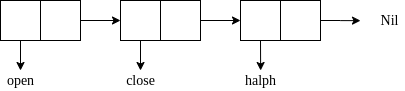
\includegraphics[scale=0.55]{pics/task11.png}}
		\caption{Решение задания 1.1.1}
	\end{figure}
	\item '((open1)(close2)(halph3));
	\begin{figure}[!h]
		\center{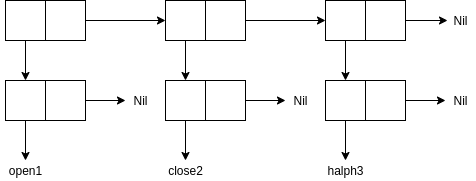
\includegraphics[scale=0.55]{pics/task12.png}}
		\caption{Решение задания 1.1.2}
	\end{figure}
	\item '((one) for all (and (me (for you))));
	\begin{figure}[!h]
		\center{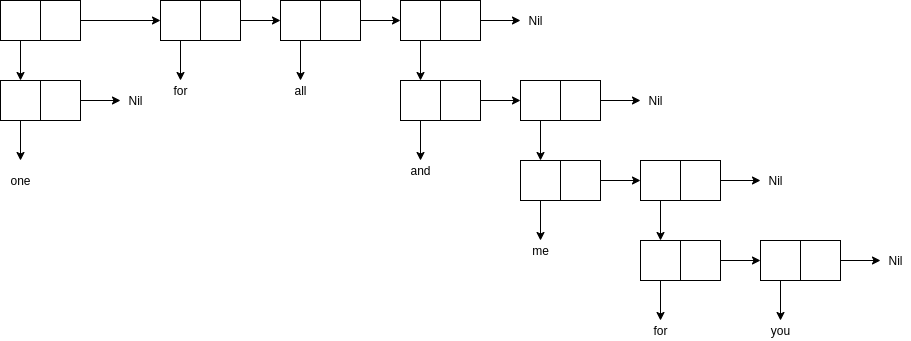
\includegraphics[scale=0.55]{pics/task13.png}}
		\caption{Решение задания 1.1.3}
	\end{figure}
	\item '((TOOL)(call));
	\begin{figure}[!h]
		\center{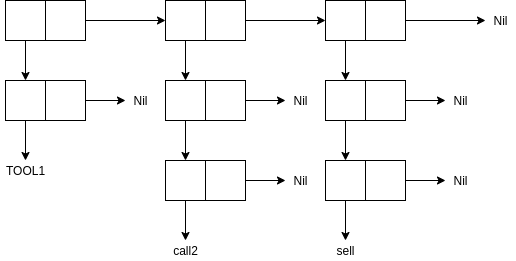
\includegraphics[scale=0.55]{pics/task15.png}}
		\caption{Решение задания 1.1.4}
	\end{figure}
	\item '((TOOL1)((call2))((sell)));
	\begin{figure}[!h]
		\center{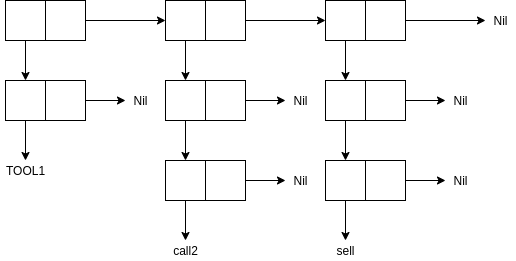
\includegraphics[scale=0.55]{pics/task15.png}}
		\caption{Решение задания 1.1.5}
	\end{figure}
	\item '(((TOOL)(call))((sell))).
	\begin{figure}[!h]
		\center{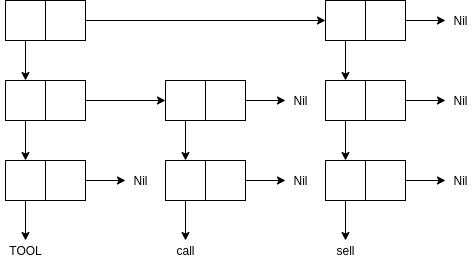
\includegraphics[scale=0.55]{pics/task16.png}}
		\caption{Решение задания 1.1.6}
	\end{figure}
\end{enumerate}

\section{Используя только функции CAR и CDR, написать выражения, возвращающие:}

\begin{enumerate}
	\item Второй элемент заданного списка: (CAR(CDR '(1 2 3 4 5)));
	\begin{figure}[!h]
		\center{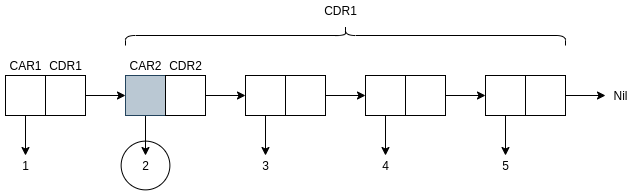
\includegraphics[scale=0.5]{pics/task21.png}}
		\caption{Решение задания 1.2.1}
	\end{figure}
	\item Третий элемент заданного списка: (CAR(CDR(CDR '(1 2 3 4 5))));
	\begin{figure}[!h]
		\center{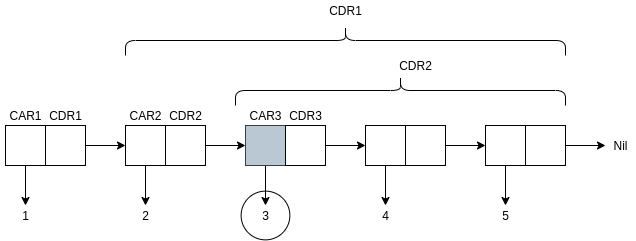
\includegraphics[scale=0.5]{pics/task22.png}}
		\caption{Решение задания 1.2.2}
	\end{figure}
	\item Четвертый элемент заданного списка: (CAR(CDR(CDR(CDR '(1 2 3 4 5))))).
	\begin{figure}[!h]
		\center{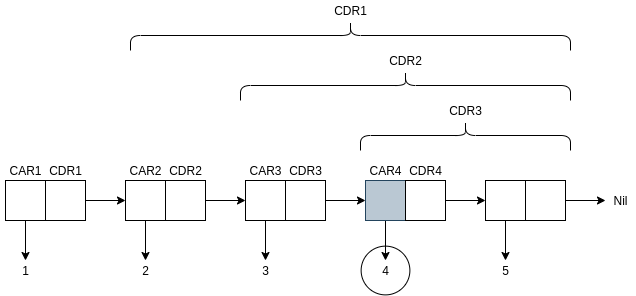
\includegraphics[scale=0.5]{pics/task23.png}}
		\caption{Решение задания 1.2.3}
	\end{figure}	
\end{enumerate}

Примечание: был задан конкретный список для примера: (1 2 3 4 5).

\section{Что будет в результате вычисления выражений?}

\begin{enumerate}
	\item (CAADR '((blue cube)(red pyramid))) $\to$ red;
	\begin{figure}[!h]
		\center{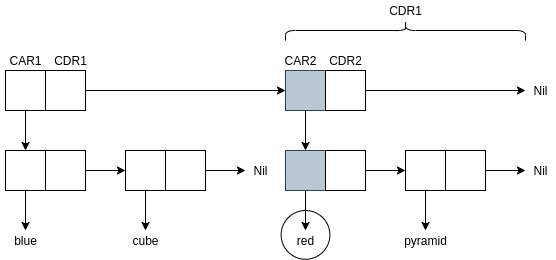
\includegraphics[scale=0.55]{pics/task31.png}}
		\caption{Решение задания 1.3.1}
	\end{figure}
	\item (CDAR '((abc)(def)(ghi))) $\to$ Nil;
	\begin{figure}[!h]
		\center{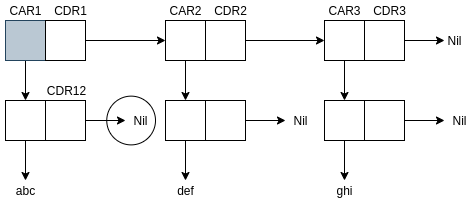
\includegraphics[scale=0.6]{pics/task32.png}}
		\caption{Решение задания 1.3.2}
	\end{figure}
	\item (CADR '((abc)(def)(ghi))) $\to$ (DEF);
	\begin{figure}[!h]
		\center{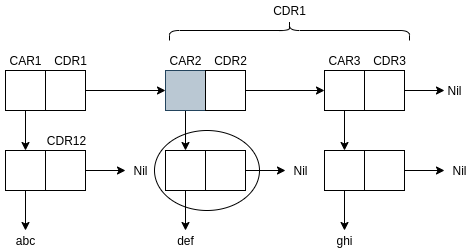
\includegraphics[scale=0.6]{pics/task33.png}}
		\caption{Решение задания 1.3.3}
	\end{figure}
	\item (CADDR '((abc)(def)(ghi))) $\to$ (GHI).
	\begin{figure}[!h]
		\center{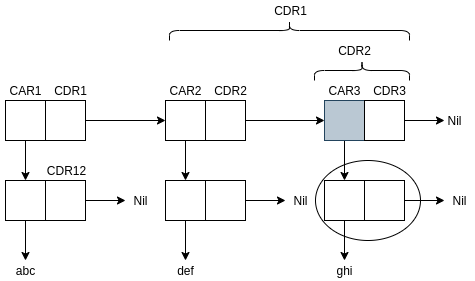
\includegraphics[scale=0.55]{pics/task34.png}}
		\caption{Решение задания 1.3.4}
	\end{figure}
\end{enumerate}

\section{Напишите результат вычисления выражений и объясните как он получен:}

[Возможно сделать отступ для объяснений письменно]

\begin{enumerate}
	\item (list 'Fred 'and 'Wilma) $\to$ (FRED AND WILMA);
	\item (list 'Fred '(and Wilma)) $\to$ (FRED (AND WILMA));
	\item (cons Nil Nil) $\to$ (NIL);
	\item (cons T Nil) $\to$ (T);
	\item (cons Nil T) $\to$ (NIL . T);
	\item (list Nil) $\to$ (NIL);
	\item (cons '(T) Nil) $\to$ ((T));
	\item (list '(one two) '(free temp)) $\to$ ((ONE TWO)(FREE TEMP));
	\item (cons 'Fred '(and Wilma)) $\to$ (FRED AND WILMA);
	\item (cons 'Fred '(Wilma)) $\to$ (FRED WILMA);
	\item (list Nil Nil) $\to$ (NIL NIL);
	\item (list T Nil) $\to$ (T NIL);
	\item (list Nil T) $\to$ (NIL T);
	\item (cons T (list Nil)) $\to$ (T NIL);
	\item (list '(T) Nil) $\to$ ((T) NIL);
	\item (cons '(one two)'(free temp)) $\to$ ((ONE TWO) FREE TEMP).
\end{enumerate}

\section{Написать лямбда-выражение и соответствующую функцию, представить результаты в виде списочных ячеек:}

\begin{enumerate}
	\item Написать функцию (f ar1 ar2 ar3 ar4), возвращающую список ((ar1 ar2)(ar3 ar4));
	\begin{figure}[!h]
		\center{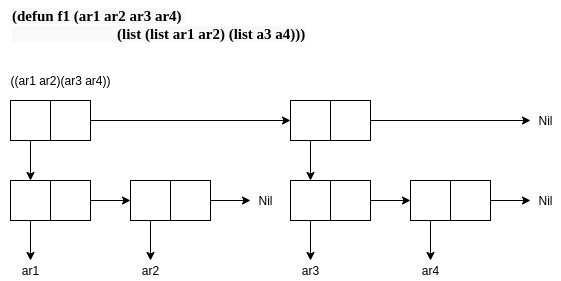
\includegraphics[scale=0.55]{pics/task51.png}}
		\caption{Решение задания 1.5.1}
	\end{figure}
	\item Написать функцию (f ar1 ar2), возвращающую список ((ar1)(ar2));
	\begin{figure}[!h]
		\center{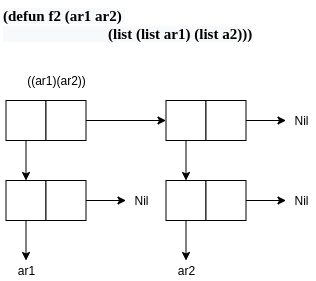
\includegraphics[scale=0.55]{pics/task52.png}}
		\caption{Решение задания 1.5.3}
	\end{figure}
	\clearpage
	\item Написать функцию (f ar1), возвращающую список (((ar1))).
	\begin{figure}[!h]
		\center{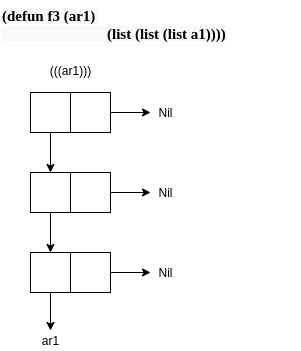
\includegraphics[scale=0.6]{pics/task53.png}}
		\caption{Решение задания 1.5.3}
	\end{figure}
\end{enumerate}
	
\end{document}